\clearpage
\section{Secure Multi-Party Computation}

\begin{refsection}

\begin{tcolorbox}	
\begin{tabular}{p{2.75cm} p{0.2cm} p{10.5cm}} 	
\textbf{Students Name}      &:& Armando Pinto (01/06/2018 - )\\
			    &:& Goncalo Vitor (15/06/2018 - )\\
                            &:& Mariana Ramos (02/05/2018 - 21/05/2018)\\
\textbf{Goal}               &:& Description of the problem of Secure Multi-Party Computation.\\
\textbf{Directory}          &:& \\
\end{tabular}
\end{tcolorbox}


\subsection{Problem definition}

In \textit{Secure Multi-Party Computation} (SMC) the function to be computed is defined as $(y_1,y_2,y_3,y_4,...,y_N)=f(x_1,x_2,x_3,x_4,...,x_N)$ and each party $i$ must only know (before and after the computation) its $x_i$ and $y_i$ being unknown any information about the input or output of the other parties. \cite{Naumann16}.

\begin{figure}[H]
	\centering
	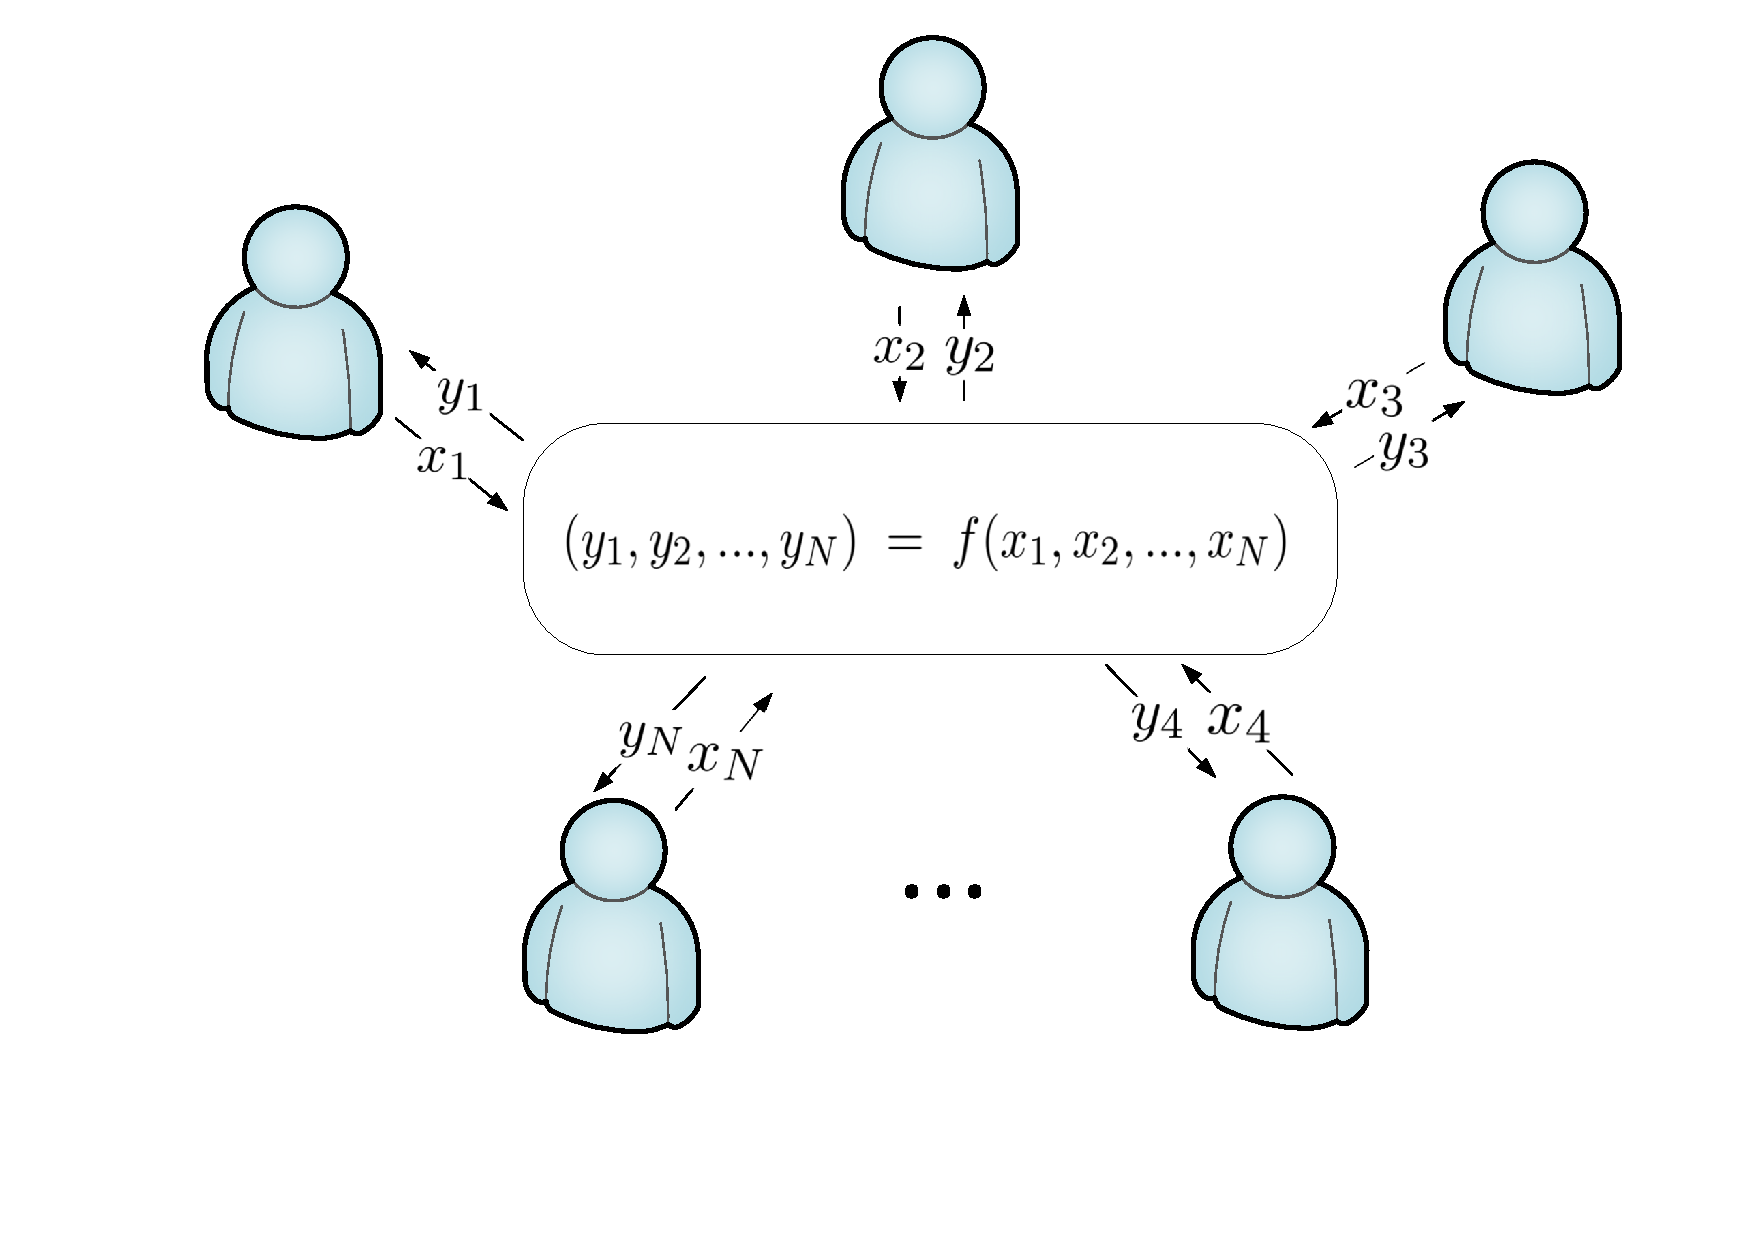
\includegraphics[width=1\textwidth, height=7cm]{./sdf/secure_multiparty_computation/figures/smc_N.pdf}
    \caption{N entities are able to jointly compute $(y_1,y_2,y_3,y_4,...,y_N)=f(x_1,x_2,x_3,x_4,...,x_N)$ making sure that each entity only have access its input/output pair, i.e. $\left( x_i, y_i\right)$.}\label0{fig:smcN}
\end{figure}

Thus, there are two ways of solving the problem of SMC:

\begin{enumerate}
  \item The result can be computed using a trusted party involved who has the trust from all the parties. This is a simple solution for the current problem, however, it requires a trusted party.
  \item The result can be computed without a trusted party involved using a SMC protocol. We are going to consider the \textit{Garbled Circuit Protocol} (GCP), which will have our best attention in this chapter.
\end{enumerate}

We will only focus on a two-party computation ($N=2$), with a single output, i.e. $y = f(x_1, x_2)$.

\subsection{Secure Two-Party Computation}

The \textit{Garbled Circuit Protocol} (GCP) starts with a transformation of the $f(x_1,x_2,...,x_N)$ function into a boolean circuit. The logical function $f_c$ is the output of the logical boolean circuit generator which implements $f(x_1,x_2,...,x_N)$. From the logical implementation, $f_c( )$, Alice will generate a garbled version of the logical function, $F_g^f$, as well as an encryption key $e_g^f$ and a decryption key $d_g^f$. After that, Alice's input parameter ($x_1$) and Bob's input parameter ($x_2$) must both be encrypted using the key $e_g^f$. Note that the encryption must be implemented with OT because Alice cannot know the Bob's input $x_2$ and Bob cannot know the encryption key, $e_g^f$, generated by Alice \cite{Naumann16}. Therefore after encryption Bob only gets $X_2$, which is its garbled input parameter. Next, Alice sends to Bob the garbled circuit, $F_g^f$, and its garbled input, $X_1$. With $F_g^f$, $X_1$ and $X_2$ Bob computes, the garbled output $Y_g^f$. With $Y_g^f$ and the decryption key $d_g^f$, Bob obtains $y=f(x_1,x_2)$. To conclude the protocol Bob will send to Alice the result $y$. Figure \ref{fig:garbledcircuit} shows the diagram of \textit{garbled circuit protocol}.

\begin{figure}[H]
	\centering
	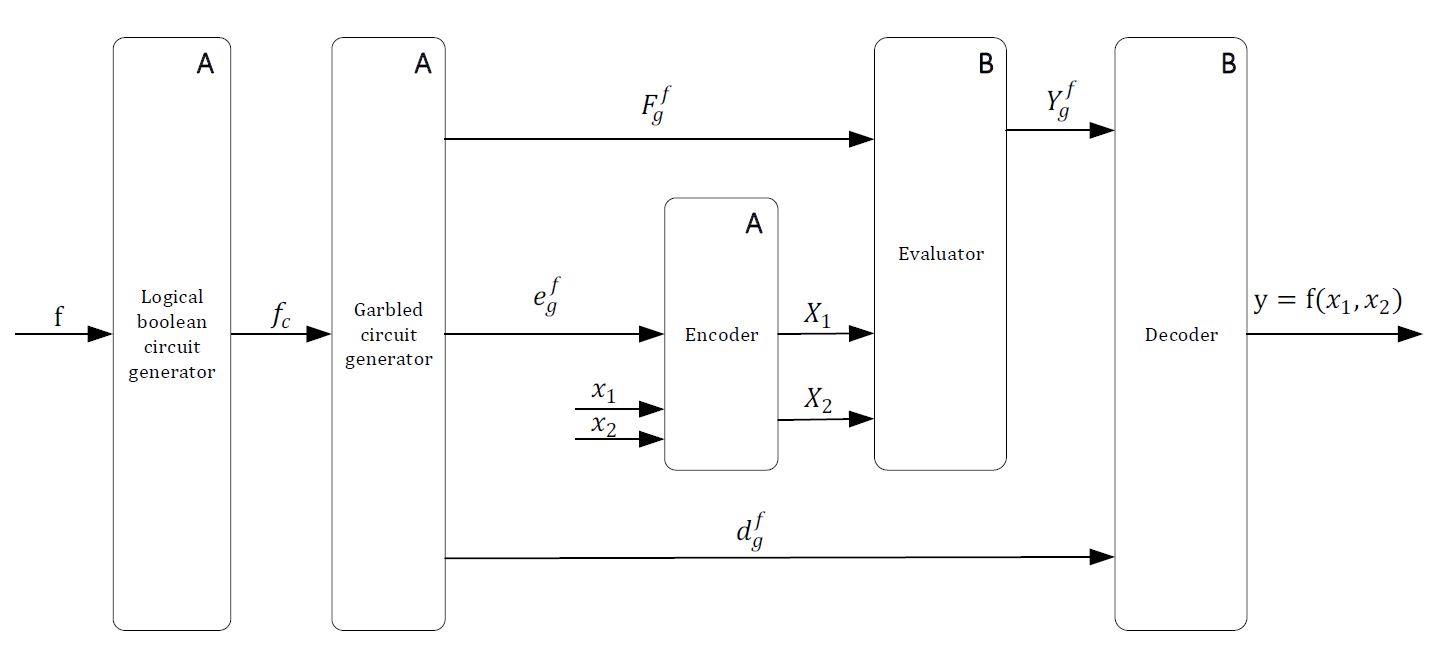
\includegraphics[width=1\textwidth, height=7cm]{./sdf/secure_multiparty_computation/figures/garbled_circuit.png}
    \caption{Block diagram of the garbled circuit protocol. Function to be computed $y=f(x_1, x_2)$. The blocks with label A are implemented by Alice and the blocks with label B are implemented by Bob.}\label{fig:garbledcircuit}
\end{figure}


\begin{table}[H]
\centering

\begin{tabular}{|c|c|}
\hline
$x_1$                   & Alice input parameter             \\ \hline
$x_2$                   & Bob input parameter               \\ \hline
$f$                     & Function to compute               \\ \hline
$f_c$                   & Logical function to be computed   \\ \hline
$F_g^f$                 & Garbled circuit of $f$            \\ \hline
$X_1$                   & Alice garbled input               \\ \hline
$X_2$                   & Bob garbled input                 \\ \hline
$e_g^f$                 & Encoding key                      \\ \hline
$d_g^f$                 & Decoding key                      \\ \hline
$Y_g^f$                 & Garbled output                    \\ \hline
\end{tabular}
\caption{Description of parameters of figure \ref{fig:garbledcircuit}.}
\end{table}




\subsubsection{Example of a two-party computation with a single output}

Lets assume:

\begin{equation}\label{eq:f_to_be_computed}
  y=f(x_1,x_2),
\end{equation}
with,

\begin{equation}\label{eq:fc_to_be_computed}
  y=f_c(x_1, x_2) = x_1 \wedge x_2,
\end{equation}
where $x_1$ and $x_2$ are single bit values. Note that even if the input parameters of $f$ and $f_c$ are represented by the same symbols they are different. The input parameters of $f_c$ are logical representations of the input parameters of $f$.

\begin{figure}[H]
	\centering
	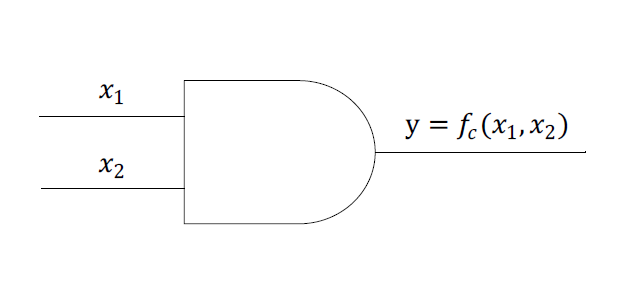
\includegraphics[width=0.4\textwidth, height=2.5cm]{./sdf/secure_multiparty_computation/figures/Gate.png}
    \caption{Gate level implementation of $f_c$.}\label{fig:andGate}
\end{figure}

Figure \ref{fig:andGate} shows the logical boolean circuit representation of the function to be computed. In this particular case there are two parties, each with an input parameter $x_i$, where $i$ can be $1$ (Alice) or $2$ (Bob), and $x_i$ can take values $0$ or $1$. Alice will play the role of \textit{garbled circuit generator} so she will generate a garbled AND gate and send it to Bob. On the other hand, Bob will play the role of \textit{garbled circuit evaluator} \cite{Yakoubov}.

\begin{figure}[H]
	\centering
	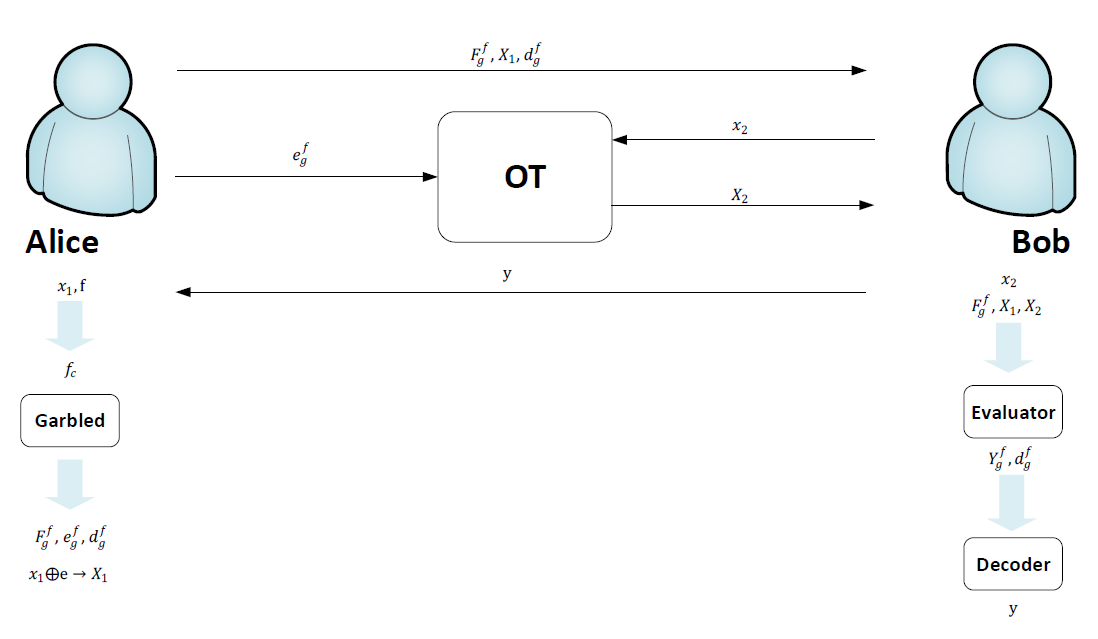
\includegraphics[width=1\textwidth, height=10cm]{./sdf/secure_multiparty_computation/figures/smc_with_ot.png}
    \caption{Garbled Circuit Protocol with OT.}\label{fig:smcwithot}
\end{figure}



\begin{table}[H]
\centering
\begin{tabular}{|c|c|c|}
\hline
$x_1$           & $x_2$             & $y=x_1 \wedge x_2$       \\ \hline
0               & 0                 & 0                             \\ \hline
0               & 1                 & 0                             \\ \hline
1               & 0                 & 0                             \\ \hline
1               & 1                 & 1                             \\ \hline
\end{tabular}
\caption{Truth table of $f_c(x_1,x_2)$.}\label{tb:truthtable}
\end{table}

Table \ref{tb:truthtable} shows the truth table of $f_c$. Initially, Alice generates an encryption key with length equals to the sum of the length of both input parameters, two bit length in this case. Then, she encrypts her two possible input parameters, $X_1 = x_1 \bigoplus e_g^f[1]$, as well as Bob's two possible input parameters, $X_2 = x_2 \bigoplus e_g^f[2]$. Lets assume $e_g^f = 01$ the encryption key used by Alice. In this case, the encryption key has two bits and Alice will use the first bit to encrypt her input parameter $x_1$ and the second bit to encrypt Bob's input parameter $x_2$. We are defining the Alice encrypted input value with the label $W_1^0$ when it before encryption assumes the value $x_1 = 0$, and $W_1^1$ when it before encryption assumes the value $x_1 = 1$. The same happens for Bob, please see table \ref{tb:aliceinputs} and \ref{tb:bobinputs}.

\begin{table}[H]
\centering
\begin{tabular}{|c|c|}
\hline
$x_1$           & $X_1 = W_1^{x_1}$                             \\ \hline
0               & $W_1^0=x_1 \bigoplus e_g^f[1] = 0$                   \\ \hline
1               & $W_1^1=x_1 \bigoplus e_g^f[1] = 1$                   \\ \hline
\end{tabular}
\caption{Encryption results for Alice's input parameter $x_1$ using the first bit of encryption key $e_g^f[1]=0$.} \label{tb:aliceinputs}
\end{table}

\begin{table}[H]
\centering
\begin{tabular}{|c|c|}
\hline
$x_2$           & $X_2 = W_2^{x_2}$                             \\ \hline
0               & $W_2^0=x_2 \bigoplus e_g^f[2] = 1$                   \\ \hline
1               & $W_2^1=x_2 \bigoplus e_g^f[2] = 0$                   \\ \hline
\end{tabular}
\caption{Encryption results for Bob's input parameter $x_1$ using the second bit of encryption key $e_g^f[2]=1$.} \label{tb:bobinputs}
\end{table}
Now, Alice computes an hash value for each combination $W_1^i$, $W_2^i$, and $y=f_c(x_1, x_2)$.
Lets assume she computed the Hash Functions and the results are the following:

\begin{table}[H]
    \centering
    \begin{tabular}{|c|c|c|c|c|c|c|}
    \hline
    $x_1$       & $W_1^i$       & $x_2$         & $W_2^i$   &     $y=f_c(x_1, x_2)$     &    $H(W_1^i,W_2^i, y)$    &    Output                             \\ \hline
    0           & 0             & 0             & 1         &  0                        & H(0,1,0)                  & 0 0 0 0 0                             \\ \hline
    0           & 0             & 1             & 0         &  0                        & H(0,0,0)                  & 0 1 0 0 0                             \\ \hline
    1           & 1             & 0             & 1         &  0                        & H(1,0,0)                  & 1 0 0 0 0                             \\ \hline
    1           & 1             & 1             & 0         &  1                        & H(1,0,1)                  & 1 1 1 0 0                             \\ \hline

    \end{tabular}
    \caption{Hash function computed and its result.}
\end{table}

Before forwarding these values to Bob, Alice also performs an encryption over these results using a decryption key with size equal to the length of the hash value, $d_g^f = 1 1 1 0 0$, $\textrm{Enc}(H(W_1^i,W_2^i,f_c )) = H(W_1^i,W_2^i,f_c) \bigoplus d_g^f $.

\begin{table}[H]
    \centering
    \begin{tabular}{|c|c|}
    \hline
    Enc($H(W_1^0,W_2^0,0)$)             &    1 1 1 0 0                                      \\ \hline
    Enc($H(W_1^0,W_2^1,0)$)             &    1 0 1 0 0                                     \\ \hline
    Enc($H(W_1^1,W_2^0,0)$)             &    0 1 1 0 0                                     \\ \hline
    Enc($H(W_1^1,W_2^1,1)$)             &    0 0 0 0 0                                     \\ \hline
    \end{tabular}
    \caption{Encrypted hash results.} \label{tb:encryptedhash}
\end{table}
 Now the rows of table \ref{tb:encryptedhash} must be permutated randomly.

\begin{table}[H]
    \centering
    \begin{tabular}{|c|c|}
    \hline
    Enc($H(W_1^0,W_2^1,0)$)             &    1 0 1 0 0                                     \\ \hline
    Enc($H(W_1^1,W_2^1,1)$)             &    0 0 0 0 0                                     \\ \hline
    Enc($H(W_1^0,W_2^0,0)$)             &    1 1 1 0 0                                     \\ \hline
    Enc($H(W_1^1,W_2^0,0)$)             &    0 1 1 0 0                                     \\ \hline
    \end{tabular}
    \caption{Permutated Garbled Circuit Output}
\end{table}


\begin{table}[H]
    \centering
    \begin{tabular}{|cc|c|}
    \hline
    $W_1^i$ & $W_2^i$   & Enc(H($W_1^i$,$W_2^i$,f ))         \\ \hline
    0       & 0         & 1 0 1 0 0                          \\
    1       & 0         & 0 0 0 0 0                          \\
    0       & 1         & 1 1 1 0 0                          \\
    1       & 1         & 0 1 1 0 0                          \\ \hline
    \end{tabular}
    \caption{Permutated Garbled Circuit.}
    \label{tb:summary}
\end{table}
Alice is going to send to Bob the permuted Garbled Circuit to Bob, i.e. table \ref{tb:summary} or a circuit that implement that table. Alice is also going to send to Bob the decryption key. Using $X_1$, that Alice also sends to Bob, and $X_2$, that Bob obtains from OT, he obtains the circuit output for that input values $(X1, X2)$. He decrypts this obtaining $H=Y \bigoplus d_g^f$, i.e. a valid hash value. After, he tries all possible outputs, doing $H(W_1^i, W_2^i, \textrm{guess y})$. The triplet $X_1$,$X_2$, $\textrm{guess y}$ that generates the correct hash value H corresponds to the right y.
After having y he send this value to Alice. Note that at the end Bob only knows $x_2$ and $y$, and Alice only knows $x_1$ and $y$.

\newpage


\subsection{ANP - Problem definition}

This is a rewritten version of the above sections. In \emph{Secure Multi-Party Computation} (SMC) a function $(y_1,y_2,y_3,y_4,...,y_N)=f(x_1,x_2,x_3,x_4,...,x_N)$ is computed, assuring that each party $i$ only know its $\left(x_i, y_i\right)$ pair, the input/output pair of all the other parties must remain unknown. \cite{Naumann16}.

\begin{figure}[H]\label{fig:smcN}
	\centering
	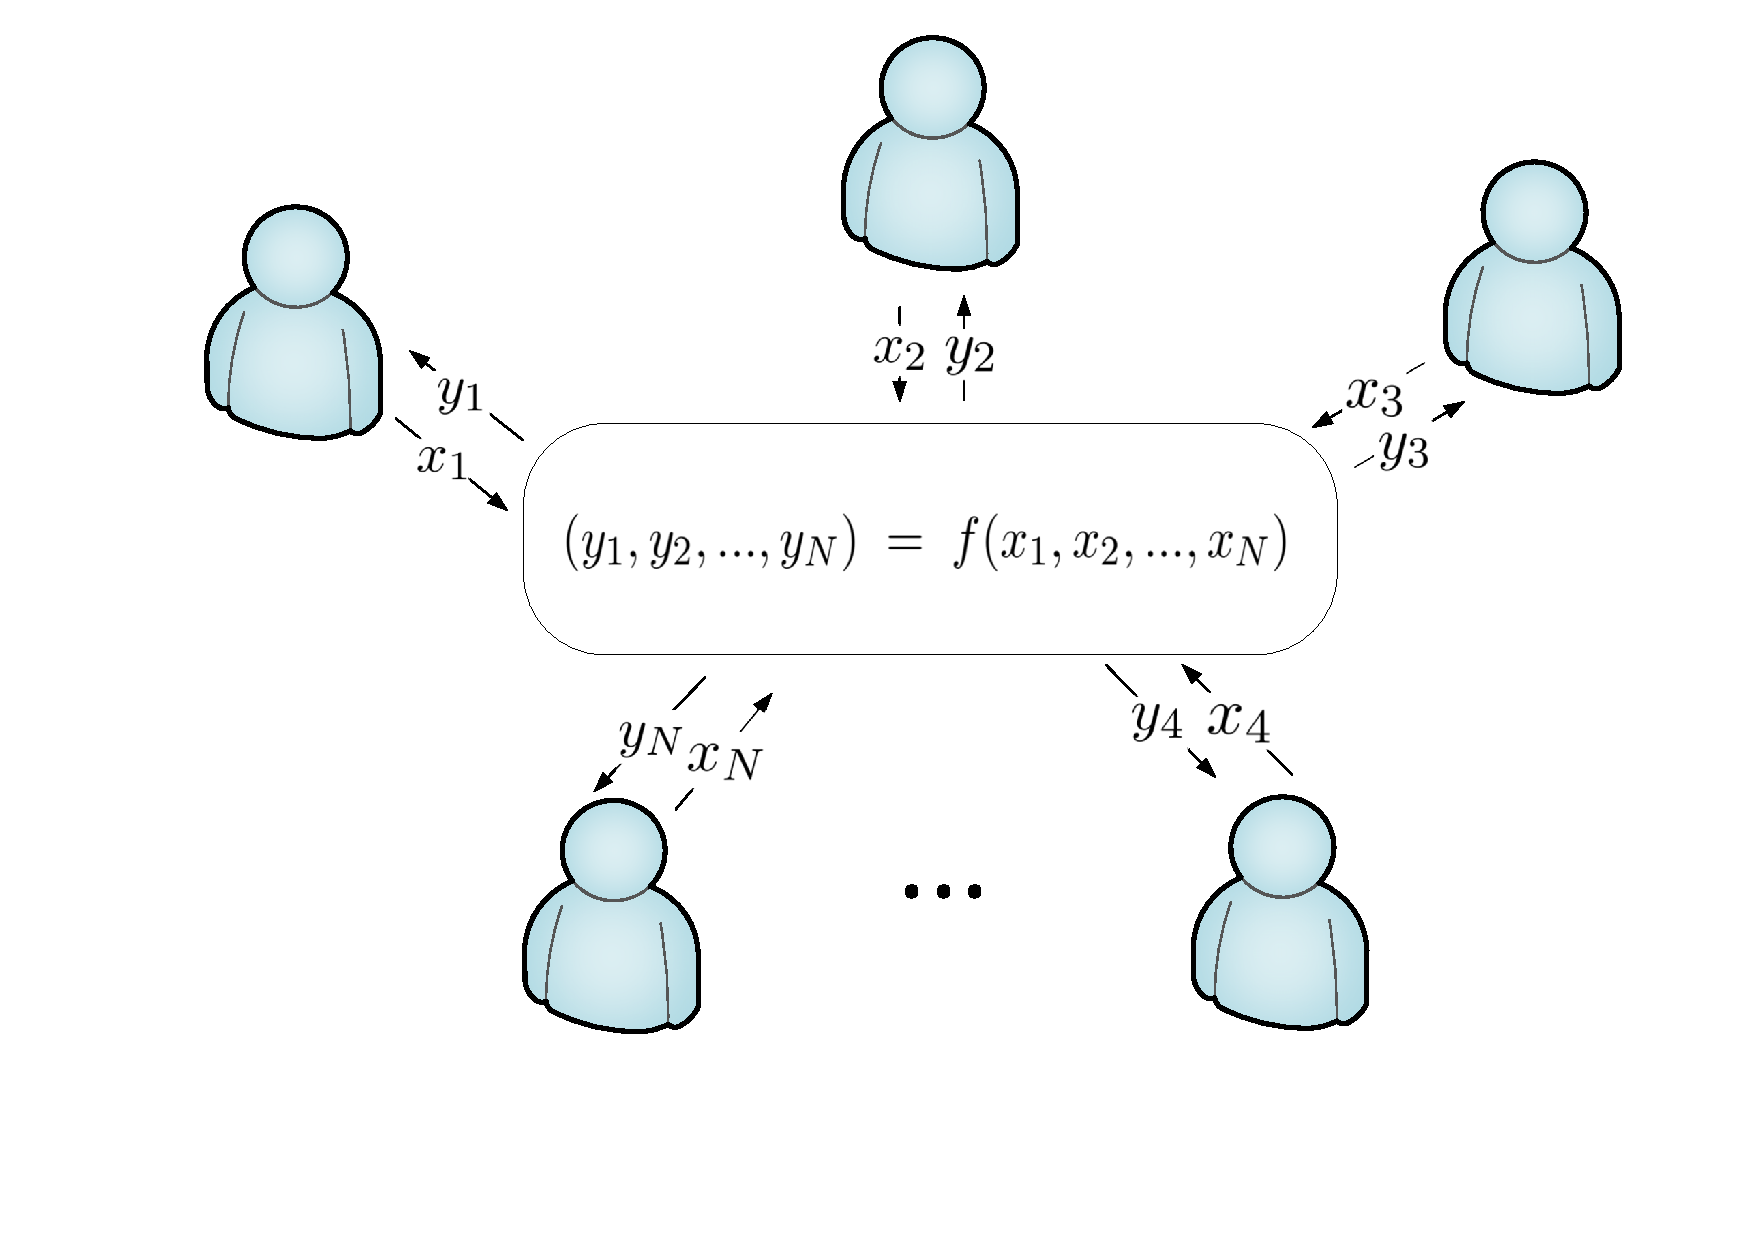
\includegraphics[width=9cm, height=7cm]{./sdf/secure_multiparty_computation/figures/smc_N.pdf}
    \caption{N entities are able to jointly compute $(y_1,y_2,y_3,y_4,...,y_N)=f(x_1,x_2,x_3,x_4,...,x_N)$ making sure that each entity only have access its input/output pair, i.e. $\left( x_i, y_i\right)$.}
\end{figure}

There are, at least, two different ways of computing this function:

\begin{enumerate}
  \item Using a trusted party, who has the trust of all the parties. This trusted party receives the all inputs, calculates the outputs and gives the the information to each party without any leak of information.
  \item Using a SMC protocol.
\end{enumerate}

Here, we are only interest in the use of a SMC protocol and we are going to restrict our work to two-party computation, with a single output, i.e. $y = f(x_1, x_2)$. For this case there is a well known protocol named \emph{Yao's Garbled Circuit Protocol} (GCP), which we are going to describe.

\subsection{ANP - Secure Two-Party Computation}

The GCP starts with the implementation of the function $f(x_1,x_2)$ using a logical circuit, i.e. using logical gates. We are going to assume that the logical circuit is implemented using NAND gates. Note that a NAND gate is a universal gate, i.e. any logical circuit can be implemented using only NAND gates. From the logical implementation, $f_c$, Alice will generate a garbled circuit, $F_g^f$, as well as an encryption key $e_g^f$ and a decryption key $d_g^f$. Because we are going to assume AES-128 as the encrypting and decrypting, which is a symmetric algorithm, both keys are identical and correspond to 128 bits. Alice's input parameter ($x_1$) and Bob's input parameter ($x_2$) must both be encrypted using the key $e_g^f$. Note that the encryption of Bob's input, $x_2$, must be implemented with OT because Alice cannot know the Bob's input, $x_2$, and Bob cannot know the encryption key, $e_g^f$, used by Alice \cite{Naumann16}. Therefore after encryption Bob only gets $X_2$, which is its encrypted input. Next, Alice sends to Bob the garbled circuit, $F_g^f$, and its encrypted input, $X_1$. With $F_g^f$, $X_1$ and $X_2$ Bob computes, the garbled output $Y_g^f$. At this stage Alice is going to send to Bob enough information so that from $Y_g^f$ he can obtain $y$. To conclude the protocol Bob will send to Alice the result $y$. Figure \ref{fig:garbledcircuit} shows the diagram of \textit{garbled circuit protocol}.

\begin{figure}[H]
	\centering
	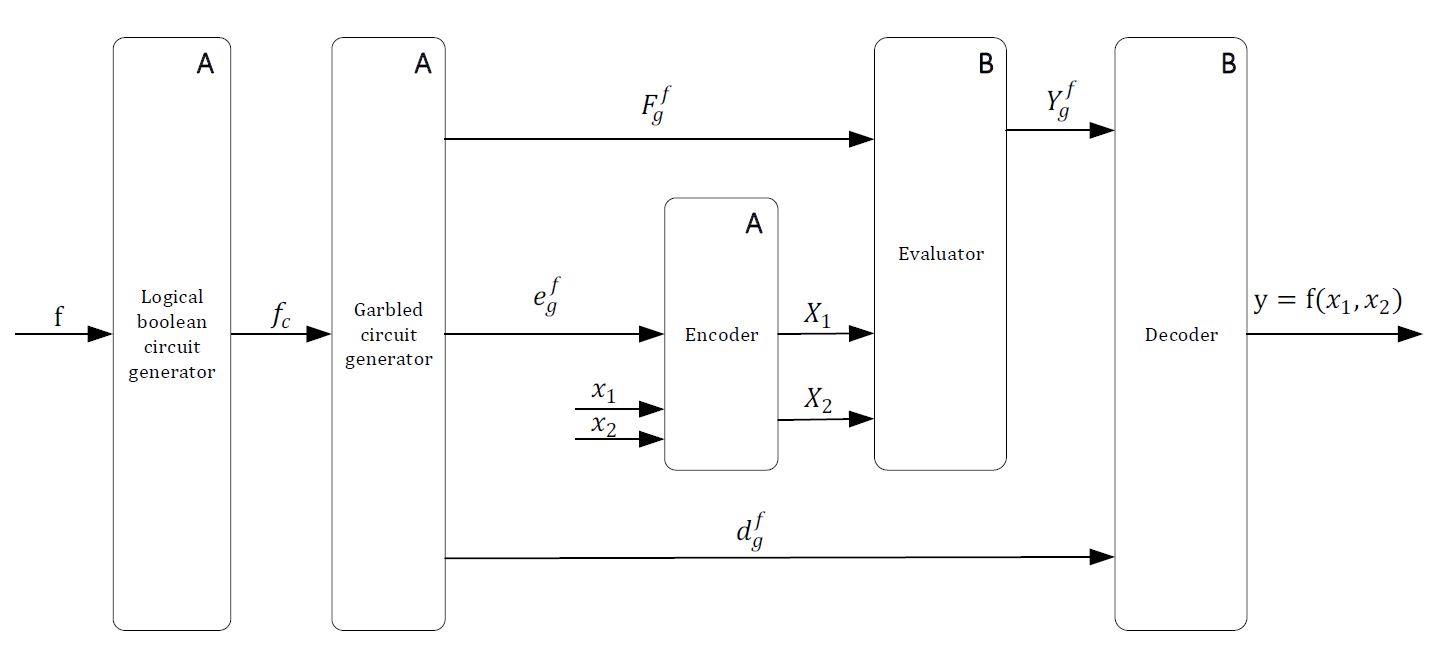
\includegraphics[width=1\textwidth, height=7cm]{./sdf/secure_multiparty_computation/figures/garbled_circuit.png}
    \caption{Block diagram of the garbled circuit protocol. Function to be computed $y~=~f(x_1, x_2)$. The blocks with label A are implemented by Alice and the blocks with label B are implemented by Bob.}\label{fig:garbledcircuit}
\end{figure}


\begin{table}[H]
\centering

\begin{tabular}{|c|c|}
\hline
$x_1$                   & Alice input parameter             \\ \hline
$x_2$                   & Bob input parameter               \\ \hline
$f$                     & Function to be computed           \\ \hline
$f_c$                   & Logical implementation            \\ \hline
$F_g^f$                 & Garbled circuit                   \\ \hline
$X_1$                   & Alice encrypted input              \\ \hline
$X_2$                   & Bob encrypted input               \\ \hline
$e_g^f$                 & Encoding key                      \\ \hline
$d_g^f$                 & Decoding key                      \\ \hline
$Y_g^f$                 & Garbled output                    \\ \hline
\end{tabular}
\caption{Description of parameters of figure \ref{fig:garbledcircuit}.}
\end{table}
%
Note that to implement the GCP, it is necessary an encryption protocol, usually AES, and an OT protocol, usually based on the RSA.


\subsubsection{Lets consider the simplest possible circuit - a NAND gate}

Lets assume:

\begin{equation}\label{eq:f_to_be_computed}
  y=f(x_1,x_2),
\end{equation}
with,

\begin{equation}\label{eq:fc_to_be_computed}
  y=f_c(x_1, x_2) = \sim \left( x_1 \wedge x_2 \right),
\end{equation}
where $x_1$ and $x_2$ are single bit values. Note that even if the input parameters of $f$ and $f_c$ are represented by the same symbols they are different. The input parameters of $f_c$ are logical representations of the input parameters of $f$.

\begin{figure}[H]
	\centering
	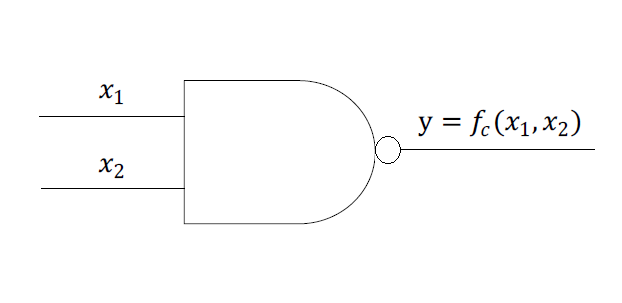
\includegraphics[width=0.4\textwidth, height=2.5cm]{./sdf/secure_multiparty_computation/figures/nand.png}
    \caption{Gate level implementation of $f_c$.}\label{fig:andGate}
\end{figure}

Figure \ref{fig:andGate} shows the logical boolean circuit representation of the function to be computed. In this particular case there are two parties, each with an input parameter $x_i$, where $i$ can be $1$ (Alice) or $2$ (Bob), and $x_i$ can take the logical value $0$ or $1$. Alice will play the role of \textit{garbled circuit generator} so she will generate a garbled NAND gate and send it to Bob. On the other hand, Bob will play the role of \textit{garbled circuit evaluator} \cite{Yakoubov}.

\begin{figure}[H]
	\centering
	\includegraphics[width=0.9\textwidth, height=15cm]{./sdf/secure_multiparty_computation/figures/smc_with_ot_ANP.png}
    \caption{Garbled Circuit Protocol with OT.}\label{fig:smcwithot}
\end{figure}



\begin{table}[H]
\centering
\begin{tabular}{|c|c|c|}
\hline
$x_1$           & $x_2$             & $y=\sim \left(x_1 \wedge x_2\right)$  \\ \hline
0               & 0                 & 1                                     \\ \hline
0               & 1                 & 1                                     \\ \hline
1               & 0                 & 1                                     \\ \hline
1               & 1                 & 0                                     \\ \hline
\end{tabular}
\caption{Truth table of $f_c(x_1,x_2)$.}\label{tb:truthtable}
\end{table}

Table \ref{tb:truthtable} shows the truth table of $f_c$.

Alice is going to use six random string, $W_0^A$, $W_1^A$, $W_0^B$, $W_1^B$, $W_0^C$, $W_1^C$ usually named labels. $W_0^A$, represents a logical zero for Alice, $W_1^A$ represents a logical one for Alice, $W_0^B$, represents a logical zero for Bob, $W_1^B$ represents a logical one for Bob.
We are going to assume that the $W_0^A$, $W_1^A$, $W_0^B$, $W_1^B$ labels are 64 bits. By concatenating two 64-bit labels Alice is going to obtain four different keys, that we are going to assume to be 128-bits AES keys, $K00 = \left[ W_0^A W_0^B \right] $, $K01 = \left[ W_0^A W_1^B \right] $, $K10 = \left[ W_1^A W_0^B \right]$ and $K11 = \left[ W_1^A W_1^B \right]$. The labels $W_0^C$, $W_1^C$ are 128 labels and are used to represent the outputs 0 and 1. Alice is going to obtain the following table:

\begin{table}[H]
\centering
\begin{tabular}{|c|c|c|}
\hline
$X_1$                 & $X_2$                   & $Y$  \\ \hline
$W_0^A$               & $W_0^B$                 & $enc_{K00} \left(W_1^C\right)$    \\ \hline
$W_0^A$               & $W_1^B$                 & $enc_{K01} \left(W_1^C\right)$    \\ \hline
$W_1^A$               & $W_0^B$                 & $enc_{K10} \left(W_1^C\right)$    \\ \hline
$W_1^A$               & $W_1^B$                 & $enc_{K11} \left(W_0^C\right)$    \\ \hline
\end{tabular}
\caption{Truth table of $f_c(x_1,x_2)$.}\label{tb:truthtable}
\end{table}

Now she apply a random permutation to the table and send the table to Bob.

\begin{table}[H]
\centering
\begin{tabular}{|c|c|c|}
\hline
$X_1$                 & $X_2$                   & $Y$  \\ \hline
$W_0^A$               & $W_0^B$                 & $enc_{K00} \left(W_1^C\right)$    \\ \hline
$W_1^A$               & $W_1^B$                 & $enc_{K11} \left(W_0^C\right)$    \\ \hline
$W_0^A$               & $W_1^B$                 & $enc_{K01} \left(W_1^C\right)$    \\ \hline
$W_1^A$               & $W_0^B$                 & $enc_{K10} \left(W_1^C\right)$    \\ \hline
\end{tabular}
\caption{Truth table of $f_c(x_1,x_2)$.}\label{tb:truthtable}
\end{table}

She is also sending to Bob the output labels, $W_0^C$ and $W_1^C$.

Finally, Alice sends to Bob her encrypted input, $W_{x_1}^A$. Note that from the label Bob cannot know nothing about $x_1$.

Bob also knows its label $W_{x_2}^B$ that he obtained through OT, therefore he can build the right key $Kx_1x_2 = \left[ W_{x_1}^A W_{x_2}^B\right]$.

He is going to apply the key to all the rows of the permuted column and he is going to obtain 4 decrypted words.
Because only one of the four decrypted words equals $W_0^C$ or $W_1^C$ Bob knows which is the output of this gate, $W_0^C$ or $W_1^C$.
Bob sends this label to Alice and Alice will tell him which was the result of the computation, 0 or 1.

Note that this is scalable for any number of gates.

\newpage

\subsection{TinyGarble}

This subsection will cover the installation and usage of TinyGarble, a GC framework that allows two parties to safely compute any function with their private inputs through Yao's Garbled Circuit Potocol. It accepts HDL and C/C++ as user inputs, although HDL will be the primary focus.

\subsubsection{Installation}

Since TinyGarble and most of the tools mentioned below have been mostly tested on Linux, it will be assumed that the user is running Linux on a virtual machine (VM), or directly from a partition. To do the former one can use Oracle's VirtualBox, which can be downloaded at \url{https://www.virtualbox.org/wiki/Downloads}. A copy of Linux is also needed, for this section Ubuntu 18.04 was used, found at \url{https://www.ubuntu.com/download/desktop}.

After installing and opening VirtualBox, select 'New', a Window should pop up asking for a name for the new VM, it doesn't matter, and for type and version, which should be Linux and Ubuntu respectively. The next step is choosing the amount of RAM that is going to be dedicated to the VM,  it depends on the system, but anything between 2048 and 4096 MB should be fine, 1024 MB or lower if the host PC has small amount of memory. Next create a virtual hard disk of VDI type, and choose dynamic or fixed size disk, it comes down to user preference. For the size of the disk, 10GB was enough to install and use TinyGarble properly, but slightly more is advisable.
After creating the virtual machine, it should ask for a start-up disk when launching it for the first time, select the Linux ISO file that was downloaded before. After that the installation of linux is pretty straight forward.

For TinyGarble to work, some dependencies have to be installed first, on Ubuntu it can be done with the following lines:

\begin{lstlisting}[caption={Installation of TinyGarble's dependencies}, language=bash, captionpos=b] 
$ sudo apt install git
$ sudo apt install build-essential
$ sudo apt install libssl1.0-dev
$ sudo apt install libboost-all-dev
$ sudo apt install cmake
\end{lstlisting}

After this step i'ts necessary to clone TinyGarble's repository, at \url{https://github.com/esonghori/TinyGarble}, and build it.

\begin{lstlisting}[caption={Configuration and compilation of TinyGarble}, language=bash, captionpos=b] 
$ git clone https://github.com/esonghori/TinyGarble.git
$ cd TinyGarble/
$ ./configure
$ cd bin/
$ make
\end{lstlisting}

To be able to use TinyGarble, a RTL Synthesis tool is also needed, to translate Verilog files into Netlist ones. In the example showed later, Yosys-abc is used. Which can be installed on Ubuntu 15.04 or higher with:

\begin{lstlisting}[caption={Installation of Yosys-abc for Ubuntu 15.04>}, language=bash, captionpos=b]                                                                                                                                                                
$ sudo apt-get install yosys
\end{lstlisting}

If on Ubuntu 14.04 or lower, a repository needs to be added first:

\begin{lstlisting}[caption={Installation of Yosys-abc for Ubuntu 14.04<}, language=bash, captionpos=b] 
$ sudo add-apt-repository ppa:saltmakrell/ppa
$ sudo apt update                                                                                                                                                                                             
$ sudo apt install yosys
\end{lstlisting}

\newpage

\subsubsection{Usage}

\begin{figure}[H]
	\centering
	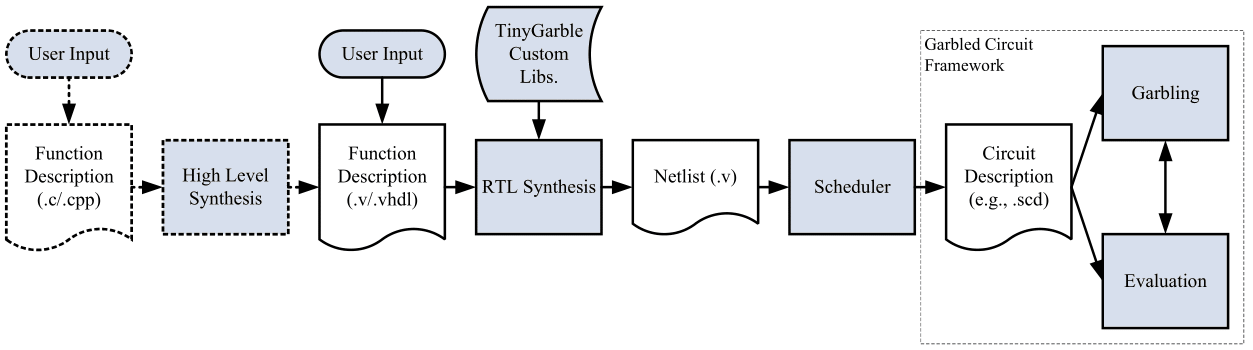
\includegraphics[width=1\textwidth, height=3cm]{./sdf/secure_multiparty_computation/figures/tiny_garble_flow.png}
    \caption{TinyGarble Global Flow\cite{Songhori}}\label{fig:tinygarble_flow}
\end{figure}

Following TinyGarble's global flow showed on the image above, it's possible to see that a C/C++ or Hardware Design Language (HDL) input is necessary. The former is slightly worse in terms of performance, since it needs an extra step of synthesis, with the help of a High Level Synthesis (HLS) tool, like Spart or Xilinx Vivado for C, to compile the C/C++ file into HDL, causing the end SCD file to have more logical gates than when using HDL input directly. This section mostly covers Verilog, since it's the most direct input, if VHDL input is needed, check \ref{ssec:usingVHDL}.

When writting the input file, some attention to the circuit's ports is needed, since TinyGarble's V2SCD (Netlist Verilog to SCD converter) accepts netlist files with a special format. 
Below are the ports that can be used and what they represent.

\begin{itemize}  
\item clk: clock cycle
\item rst: active high reset
\item g\_init: garbler's initial values (read at the first clock)
\item e\_init: evaluator's initial values (read at the first clock)
\item g\_input: garbler's input (read at every clock)
\item e\_input: evaluator's input (read at every clock)
\item o: output
\end{itemize}

Below it's an example of an and\_gate written in verilog with the format above.

\begin{lstlisting}[caption={and\_gate.v}, language=Verilog, captionpos=b] 
module and_gate (input g_input, e_input, output o);
	assign o = g_input & e_input;
endmodule
\end{lstlisting}

Using TinyGarble's custom library, asic\_cell\_yosys\_extended.lib", located at TinyGarble/ciruit\_synthesis/lib/, and assuming that the Verilog file is located at a folder named "circuits", the compilation can be done with the following instructions:

\begin{lstlisting}[caption={Yosys instructions to compile the HDL file to a Netlist file}, language=bash, captionpos=b] 
$ ./yosys
yosys> read_verilog circuits/and_gate.v
yosys> hierarchy -check -top and_gate
yosys> proc; opt; memory; opt; fsm; opt; techmap; opt;
yosys> abc -liberty TinyGarble/circuit_synthesis/lib/
asic_cell_extended.lib
yosys> clean
yosys> write_verilog circuits/and_gate_netlist.v
yosys> exit					
\end{lstlisting}

Following these, the Netlist file below should be generated.

\begin{lstlisting}[caption={and\_gate\_netlist.v}, language=Verilog, captionpos=b] 
(* top =  1  *)
(* src = "and.v:1" *)
module and_gate( g_input,  e_input, o);
  (* src = "and.v:2" *)
  input g_input;
  (* src = "and.v:2" *)
  input e_input;
  (* src = "and.v:3" *)
  output o;
  AND _0_ (
    .A(e_input),
    .B(g_input),
    .Z(o)
  );
endmodule
\end{lstlisting}

For some unkown reason, the output file has some noticeably weird lines, starting with "(*", that will cause Segmentation Fault error in the next step if not removed.
After removing those lines, the Netlist file can be converted into a SCD file with the instruction below:

\begin{lstlisting}[caption={Installation of Yosys-abc}, language=bash, captionpos=b] 
$ ./TinyGarble/bin/scd/V2SCD_Main -i circuits/and_gate_netlist.v 
-o circuits/and_gate.scd		
\end{lstlisting}

Before executing the SCD file, it can be tested with TinyGarble's SCD\_Evaluator\_Main located at TinyGarble/bin/scd, with the code below:

\begin{lstlisting}[caption={Testing a SCD file}, language=bash, captionpos=b] 
$ ./TinyGarble/bin/scd/SCD_Evaluator_Main -i circuits/and_gate --g_input 1 --e_input 0
\end{lstlisting}

\newpage

The SCD file can now be executed by both parties, "Alice" and "Bob", as shown on the upper terminal and lower terminal of the following images, respectively.
For this examples the SCD file was located at TinyGarble/bin/garbled\_circuits, same directory where the instructions were executed.

\begin{figure}[H]
	\centering
	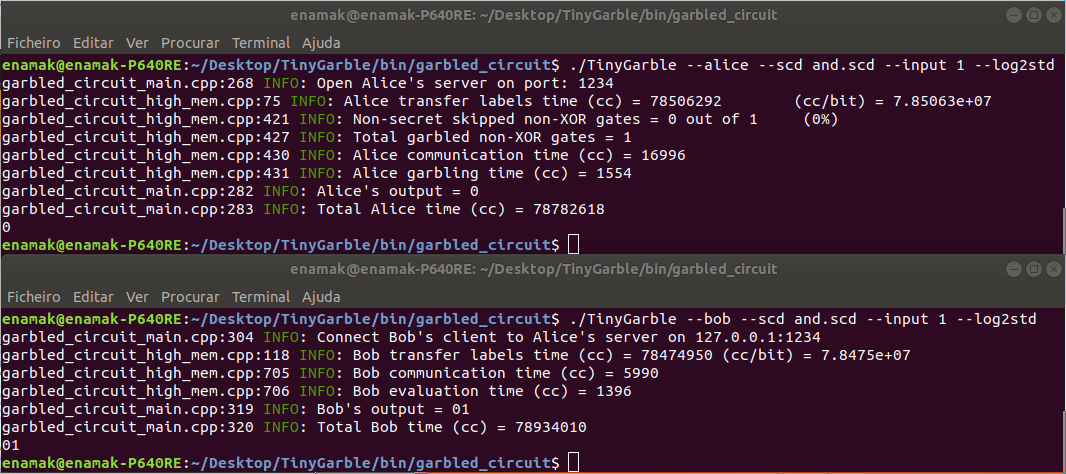
\includegraphics[width=1\textwidth, height=7cm]{./sdf/secure_multiparty_computation/figures/tinygarble_and_a.png}
    \caption{"And" function executed by Alice and Bob, with inputs 1 and 1, respectively}\label{fig:tinygarble_and_a}
\end{figure}

\begin{figure}[H]
	\centering
	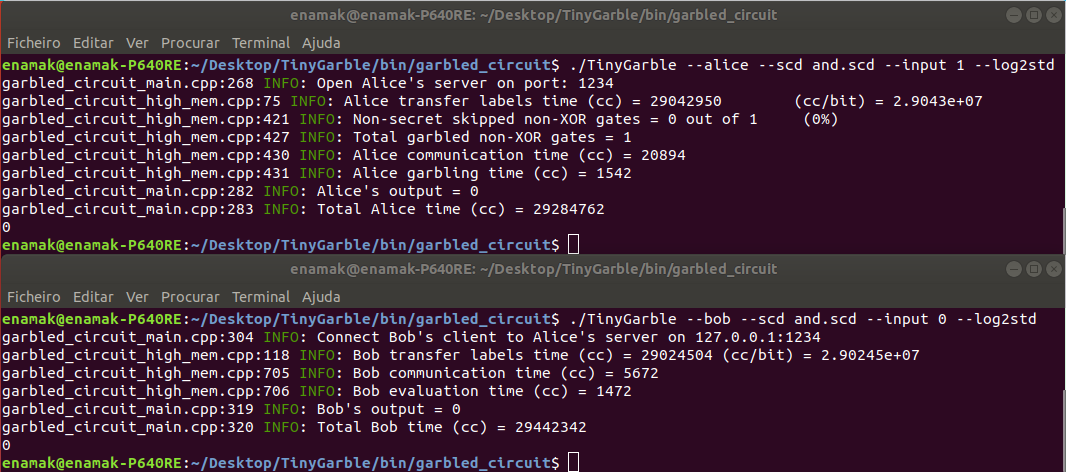
\includegraphics[width=1\textwidth, height=7cm]{./sdf/secure_multiparty_computation/figures/tinygarble_and_b.png}
    \caption{"And" function executed by Alice and Bob, with inputs 1 and 0, respectively}\label{fig:tinygarble_and_b}
\end{figure}

The input is written in hexadecimal, and the log2std option is to show information of the computation on the terminal instead of creating a log file.

\begin{figure}[H]
	\centering
	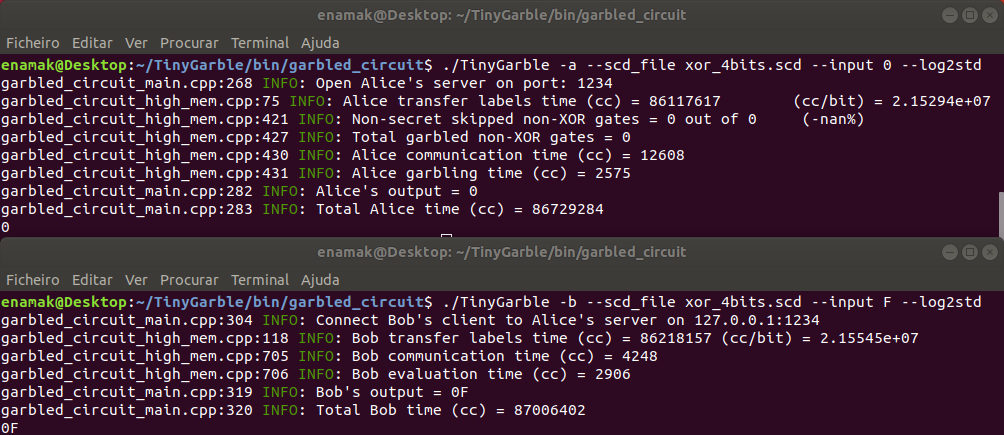
\includegraphics[width=1\textwidth, height=7cm]{./sdf/secure_multiparty_computation/figures/tinygarble_xor_4bits_b.png}
    \caption{"Xor" function with 4 bits, executed by Alice and Bob, with inputs 0 and F, respectively}\label{fig:tinygarble_xor_b}
\end{figure}

\subsubsection{Using VHDL} \label({ssec:usingVHDL}

If the desirable input is VHDL, this next tool, V2VHDL, will be necessary to translate it into Verilog, which is the input supported by the RTL Synthesis Tool mentioned before.
Before cloning vhd2vl at \url{https://github.com/ldoolitt/vhd2vl} and building it, some dependencies have to be installed:

\begin{lstlisting}[caption={Installation of VHD2VL}, language=bash, captionpos=b]                                                                                                                                                                                  
$ sudo apt install flex                                                                                                                                                                         
$ sudo apt install bison
$ git clone https://github.com/ldoolitt/vhd2vl
$ cd vhd2vl/src
$ make
$ sudo cp vhd2vl /usr/local/bin
\end{lstlisting}

To use it simply run:

\begin{lstlisting}[caption={Translation of VHDL file into Verilog}, language=bash, captionpos=b] 
$ vhd2vl and_gate.vhd and_gate.v	
\end{lstlisting}

\newpage

\subsubsection{Programming}

\subsubsection{File Architecture}

\begin{enumerate}
\item a23: Algorithms wrote in C.
\item bin: Created when building TinyGarble. Holds executables and examples of netlist and scd files.
\item circuit\_synthesis: Holds netlist and RTL Verilog files and the custom libs to use with Yosys.
\item crypto: Holds C++ files for the Oblivious Transfer and their data structure, 'block'.
\item garbled\_circuit: Holds C++ files to deal with the garbling and evaluation of a circuit.
\item scd:  Holds C++ files of the SCD Converter and Evaluator mentioned before, and of the netlist Parser.
\item tcpip: Holds C++ files that deal with server connection.
\item util: Holds C++ support files.
\end{enumerate}

\subsubsection{Keys}

Since TinyGarble is based on JustGarble, it's garbling scheme will be based on fixed-key AES. If the user wants to use his own encryption and decryption keys, the "garbled\_circuit.cpp" file located at "TinyGarble/garbled\_circuit" has to be slightly changed. For this example, both the garbler and evaluator get their keys from their respective file, to accomplish this, on GarbleStr and EvaluateStr functions, change the line "block global\_key =  RandomBlock();" with the code below:

\begin{figure}[H]
	\centering
	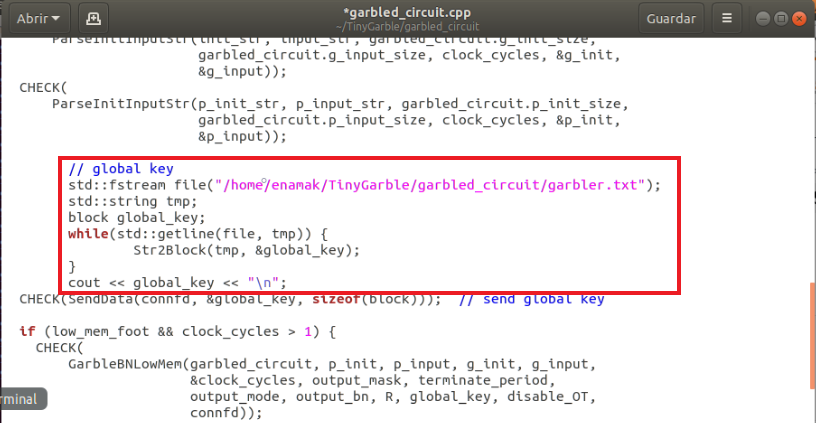
\includegraphics[width=1\textwidth, height=5.5cm]{./sdf/secure_multiparty_computation/figures/key_file.png}
    \caption{Reading Garbler's key from a file.}\label{fig:key_file}
\end{figure}

The figure above is showing a piece of the modified GarbleStr function, the same would have to be done at the EvaluatorStr function with the respective path for the evaluator keys. The absolute(starting from the root) path has to be given. "\#Include <fstream>" is also needed at the top of the file.

To apply any changes made to the file, go to TinyGarble/bin and run the "make" command.

\subsubsection{Moda function}

Since the input of the function both for Alice and Bob is a series of numbers, and since TinyGarble's iinput is in hexadecimal, we can read each digit as bcd, and easily get the total by multiplying the current number by 10 and summing the digit. Instead of using a ',' any value beetween a and f can be used.

The following fucntion was wriitten in VHDL:

\begin{lstlisting}[caption={moda.vhd}, language=Verilog, captionpos=b] 

module moda(clk,  rst, g_input, e_input, o);

  input clk,  rst;
  input [1023:0] g_input, e_input; // Up to 256 hexa chars, sent from the testbench
  output [8:0] o; // With 256 hexa chars the max of different numbers is 512 (256 / 2 (commas) * 4)

  wire clk,  rst;
  reg [8:0] o;

  reg [9:0] g_iterator, e_iterator; // Represent up to the number 1023, to iterate the inputs
  wire [3:0] g_tmp, e_tmp; // To hold the current hexa char beeing checked
  reg [29:0] g_number, e_number; // Maximum of around 1 trillion, (10 hexa digits, because in bcd)
  reg g_end, e_end, g_start, e_start, g_blocked, e_blocked; // Control registers

  reg [30:0] bigger; // Hold the bigger number, one bit bigger than the biggest number for the inputs
  reg [8:0] biggerKey, counter; // Same as output

  reg [2:0] State; 

  // Wires, constantly receiving the current value of their corresponding input with the current interator
  assign g_tmp = g_input[g_iterator -: 4]; // -: notacao SystemVerilog, ver se funcioa com yosys 
  assign e_tmp = e_input[e_iterator -: 4];


always @(posedge clk) begin

	
    if ( rst) begin
      State <= 0;
      o = 0;
    end else begin

	    case(State)
	    0 : begin

		g_iterator <= 1023;
		e_iterator <= 1023;
		g_number <= 0;
		e_number <= 0;
		g_blocked <= 0;
		e_blocked <= 0;

		g_end <= 0;
		e_end <= 0;

		bigger <= 0;
		biggerKey <= 0;
		counter <= 0;

		State <= 1;

	    end
	    1 : begin
	      // Se ainda nao tiver chegado ao ultimo digito it ao proximo
	      if(g_blocked == 0) begin
		if(g_iterator < 4)
		  g_end <= 1;
		else
		  g_iterator <= g_iterator - 4;
	      end
	      if(e_blocked == 0) begin
		if(e_iterator < 4)
		  e_end <= 1;
		else begin
		  e_iterator <= e_iterator - 4;
		end
	      end
	      State <= 2;
	    end
	    2 : begin
	      if(g_blocked == 1 & e_blocked == 1)
		State <= 3;
	      else begin
		if(g_tmp == 10 | g_end == 1) 
		  g_blocked <= 1;
		else
		  g_number <= (g_number * 10) + g_tmp;
		if(e_tmp == 10 | e_end == 1) 
		  e_blocked <= 1;
		else 
		  e_number <= (e_number * 10) + e_tmp;
		State <= 1;
	      end;
	    end
	    3 : begin
	      if(g_number + e_number > bigger) begin
		$display("Found bigger");
		bigger <= g_number + e_number;
		biggerKey <= counter;
	      end
	      counter <= counter + 1;
	      g_number <= 0;
	      g_blocked <= 0;
	      e_number <= 0;
	      e_blocked <= 0;
	      if(g_end == 1 & e_end == 1) begin
		State <= 4;
	      end else 
		State <= 1;
	    end
	    4 : begin
	      o <= biggerKey + 1;
	      State <= 4;
	    end
	    default : begin
	      State <= 0;
	    end
	    endcase
	end			
  end

endmodule

\end{lstlisting}

When running a testbench of the above with the g\_input = 80'h421a425a9a23a412a432, and e\_input = 80'h94a420a83a902a74a821,  the result is the below:

\begin{figure}[H]
	\centering
	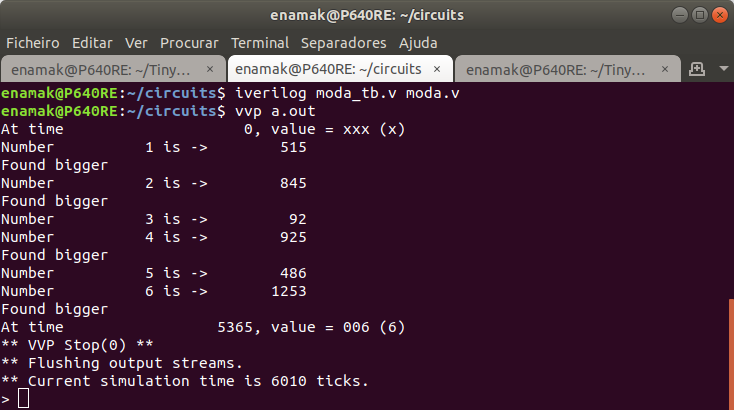
\includegraphics[width=1\textwidth, height=7cm]{./sdf/secure_multiparty_computation/figures/moda_execution_testbench.png}
    \caption{Moda's testbench execution}\label{fig:moda_execution}
\end{figure}

Converting the file to Netlist Verilog wasnt a problem besides having to delete all those weird lines mentioned above.
When trying to converto to Scd it gives the error:

\begin{figure}[H]
	\centering
	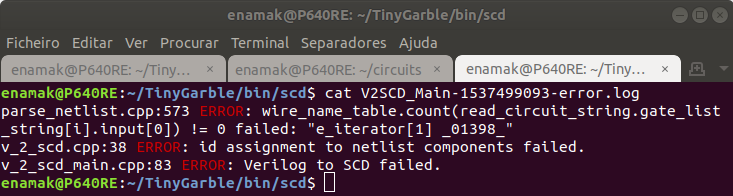
\includegraphics[width=1\textwidth, height=4cm]{./sdf/secure_multiparty_computation/figures/tinygarble_moda_scd_fail.png}
    \caption{Model SCD conversion fail}\label{fig:moda_scd_fail}
\end{figure}


% bibliographic references for the section ----------------------------
\clearpage
\printbibliography[heading=subbibliography]
\end{refsection}
\addcontentsline{toc}{subsection}{Bibliography}
\cleardoublepage
% -------------------------------------------------------------------- 
